\documentclass[12pt,a4paper]{article}

% ─── Page Layout ───────────────────────────────────────────────────────────────
\usepackage[a4paper, margin=0.8in, headheight=14pt]{geometry}

% ─── Fonts (XeLaTeX) ───────────────────────────────────────────────────────────
\usepackage{fontspec}
\usepackage{unicode-math}
\setmainfont{TeX Gyre Pagella}
\setmonofont[Scale=0.88]{TeX Gyre Cursor}
\setmathfont{Latin Modern Math}

% ─── Packages ──────────────────────────────────────────────────────────────────
\usepackage{xcolor}
\usepackage{colortbl}
\usepackage{titlesec}
\usepackage{enumitem}
\usepackage{tabularx}
\usepackage{booktabs}
\usepackage{array}
\usepackage{amsmath}
\usepackage{tikz}
\usetikzlibrary{shapes.geometric, arrows.meta, positioning, calc, fit, decorations.pathreplacing, patterns}
\usepackage{tcolorbox}
\tcbuselibrary{skins, breakable}
\usepackage{hyperref}
\usepackage{fancyhdr}
\usepackage{graphicx}
\usepackage{microtype}
\hyphenpenalty=10000
\exhyphenpenalty=10000
\sloppy
\usepackage{caption}
\usepackage{setspace}
\usepackage{multirow}
\usepackage{tocloft}

% ─── Q&A helper ────────────────────────────────────────────────────────────────
\newcommand{\Q}[1]{\textbf{#1}\par\noindent\ignorespaces}

% ─── Colour Palette ────────────────────────────────────────────────────────────
\definecolor{myred}{RGB}{196,30,58}
\definecolor{mydark}{RGB}{30,30,50}
\definecolor{mygreen}{RGB}{14,120,80}
\definecolor{myteal}{RGB}{0,130,140}
\definecolor{myamber}{RGB}{180,100,0}
\definecolor{mypurple}{RGB}{100,30,160}
\definecolor{mygray}{RGB}{246,247,249}
\definecolor{mgframe}{RGB}{180,185,200}
\definecolor{watermark}{RGB}{145,150,170}
\definecolor{hdrred}{RGB}{250,232,235}
\definecolor{hdrgreen}{RGB}{220,244,233}
\definecolor{hdrteal}{RGB}{220,242,244}
\definecolor{hdramber}{RGB}{253,242,215}
\definecolor{hdrpurple}{RGB}{238,228,255}
\definecolor{hdrgray}{RGB}{238,240,245}
\definecolor{rowalt}{RGB}{250,251,253}

% ─── Section Formatting ────────────────────────────────────────────────────────
\titleformat{\section}{\large\bfseries\color{myred}}{\thesection.}{0.5em}{}[\vspace{1pt}{\color{myred}\rule{\linewidth}{0.8pt}}]
\titleformat{\subsection}{\normalsize\bfseries\color{myteal}}{\thesubsection}{0.5em}{}
\titlespacing*{\section}{0pt}{18pt}{7pt}
\titlespacing*{\subsection}{0pt}{11pt}{4pt}

% ─── Paragraph ─────────────────────────────────────────────────────────────────
\setlength{\parindent}{0pt}
\setlength{\parskip}{4pt}

% ─── TOC Styling ───────────────────────────────────────────────────────────────
\renewcommand{\cfttoctitlefont}{\large\bfseries\color{myred}}
\renewcommand{\cftaftertoctitle}{\par\noindent{\color{myred}\rule{\linewidth}{0.8pt}}}
\setlength{\cftbeforetoctitleskip}{0pt}
\setlength{\cftaftertoctitleskip}{6pt}
\renewcommand{\cftsecfont}{\normalsize\bfseries\color{mydark}}
\renewcommand{\cftsecpagefont}{\normalsize\bfseries\color{mydark}}
\renewcommand{\cftsecleader}{\cftdotfill{\cftdotsep}}
\setlength{\cftbeforesecskip}{7pt}
\renewcommand{\cftsubsecfont}{\small\color{mydark}}
\renewcommand{\cftsubsecpagefont}{\small\color{mydark}}
\setlength{\cftbeforesubsecskip}{3pt}
\setlength{\cftsubsecindent}{1.4em}

% ─── Table helpers ─────────────────────────────────────────────────────────────
\renewcommand{\arraystretch}{1.45}
\setlength{\tabcolsep}{6pt}
\arrayrulecolor{mydark}
\newcolumntype{B}[1]{>{\small\bfseries\raggedright\arraybackslash}m{#1}}
\newcolumntype{Y}{>{\small\raggedright\arraybackslash}X}
\renewcommand{\tabularxcolumn}[1]{m{#1}}

% ─── Header / Footer ───────────────────────────────────────────────────────────
\pagestyle{fancy}
\fancyhf{}
\fancyhead[L]{\small\color{myred}\textbf{OE-EC803B}\;\color{mydark}--- Big Data Analysis}
\fancyhead[R]{\small\color{myteal}\textbf{Module 5 Notes}}
\fancyfoot[C]{\small\color{mydark}\thepage}
\fancyfoot[R]{\small\color{watermark}\textit{\copyright\ Biraj Sarkar}}
\renewcommand{\headrulewidth}{0.5pt}
\renewcommand{\footrulewidth}{0.3pt}

% ─── Hyperref ──────────────────────────────────────────────────────────────────
\hypersetup{colorlinks=true, linkcolor=myteal, urlcolor=myteal,
  pdfauthor={Biraj Sarkar}, pdftitle={OE-EC803B --- Module 5 Notes}}

% ─── tcolorbox styles ──────────────────────────────────────────────────────────
\tcbset{
  tikzbox/.style={colback=mygray, colframe=mgframe, boxrule=0.6pt, arc=4pt,
    left=8pt, right=8pt, top=6pt, bottom=6pt,
    colbacktitle=mgframe, coltitle=mydark, fonttitle=\small\bfseries, unbreakable},
  defbox/.style={colback=hdrgreen, colframe=mygreen, boxrule=0.8pt, arc=4pt,
    left=9pt, right=9pt, top=6pt, bottom=6pt,
    colbacktitle=mygreen, coltitle=white, fonttitle=\small\bfseries},
  formulabox/.style={colback=hdrteal, colframe=myteal, boxrule=0.8pt, arc=4pt,
    left=9pt, right=9pt, top=7pt, bottom=7pt,
    colbacktitle=myteal, coltitle=white, fonttitle=\small\bfseries},
  examplebox/.style={colback=hdramber, colframe=myamber, boxrule=0.8pt, arc=4pt,
    left=9pt, right=9pt, top=6pt, bottom=6pt,
    colbacktitle=myamber, coltitle=white, fonttitle=\small\bfseries},
  masonbox/.style={colback=hdrpurple, colframe=mypurple, boxrule=0.8pt, arc=4pt,
    left=9pt, right=9pt, top=6pt, bottom=6pt,
    colbacktitle=mypurple, coltitle=white, fonttitle=\small\bfseries},
  exambox/.style={colback=hdrpurple, colframe=mypurple, boxrule=1pt, arc=5pt,
    left=10pt, right=10pt, top=8pt, bottom=8pt,
    colbacktitle=mypurple, coltitle=white, fonttitle=\bfseries,
    breakable, title after break={\textbf{Frequently Asked / Viva Questions (contd.)}}}
}
\tcbset{breakable}

% ─── TikZ styles ───────────────────────────────────────────────────────────────
\tikzset{
  block/.style={rectangle, draw=myteal, fill=hdrteal,
    text width=2.2cm, align=center, minimum height=0.9cm,
    font=\small, rounded corners=3pt, line width=0.7pt},
  redblock/.style={rectangle, draw=myred, fill=hdrred,
    text width=2.2cm, align=center, minimum height=0.9cm,
    font=\small, rounded corners=3pt, line width=0.7pt},
  arrow/.style={-Stealth, thick, color=mydark},
  redarrow/.style={-Stealth, thick, color=myred},
  line/.style={thick, color=mydark}
}

\begin{document}

% ═══════════════════════════════════════════════════════════════════════════════
% TITLE BLOCK
% ═══════════════════════════════════════════════════════════════════════════════
\begin{center}
  \hfill \textit{Exam-Ready Short Notes} \\
  \vspace{6pt}
  {\LARGE\bfseries\color{myred} OE-EC803B --- Big Data Analysis}\\[5pt]
  {\normalsize\color{mydark} Semester VIII \quad$\bullet$\quad 3L:0T:0P \quad$\bullet$\quad 3 Credits}\\[3pt]
  {\normalsize\color{myteal}\textbf{Module 5: Data Analytics with R \& Machine Learning Algorithms}}\\[3pt]
  {\small\color{mydark} CGEC \;$|$\; B.Tech ECE (2023--27) \;$|$\; \textit{Biraj Sarkar}}
\end{center}
\vspace{2pt}
\noindent{\color{myred}\rule{\linewidth}{1.5pt}}
\vspace{2pt}

\hypersetup{linkcolor=mydark}
\tableofcontents
\hypersetup{linkcolor=myteal}
\newpage

% ===============================================================================
\section{R and Machine Learning in Big Data}
% ===============================================================================

Data analytics turns raw database bits into business value. R is a popular programming language for statistical computing and graphics. In Big Data architectures, statistical models are divided into supervised and unsupervised techniques:

\begin{tcolorbox}[defbox, title={Machine Learning Paradigms}]
  \begin{itemize}[leftmargin=*, itemsep=3pt]
    \item \textbf{Supervised Learning:} Training models using labeled datasets where the input features ($X$) are mapped to a known target variable ($Y$).
    \item \textbf{Unsupervised Learning:} Identifying hidden patterns, groups, or structures in unlabeled datasets where only input features ($X$) are provided.
  \end{itemize}
\end{tcolorbox}

\begin{tcolorbox}[tikzbox, title={Taxonomy of Machine Learning}]
\centering
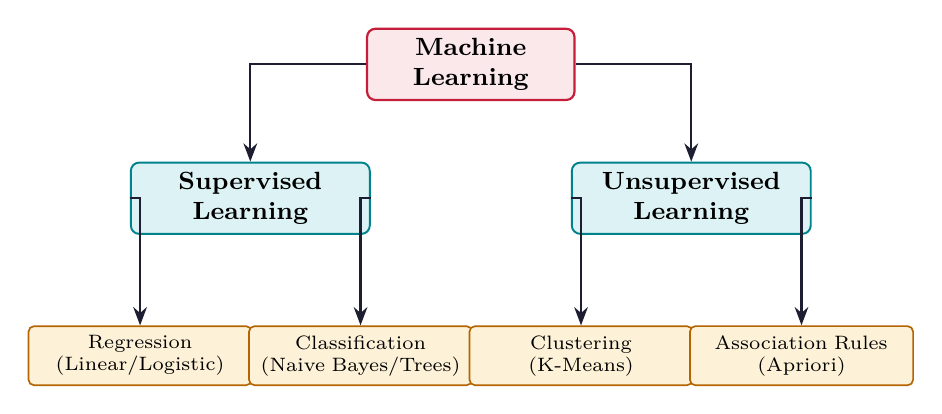
\begin{tikzpicture}[node distance=0.8cm and 0.4cm,
  root/.style={rectangle, draw=myred, fill=hdrred, text width=2.4cm, align=center, minimum height=0.8cm, font=\small\bfseries, rounded corners=3pt, line width=0.8pt},
  branch/.style={rectangle, draw=myteal, fill=hdrteal, text width=2.8cm, align=center, minimum height=0.75cm, font=\small\bfseries, rounded corners=3pt, line width=0.7pt},
  leaf/.style={rectangle, draw=myamber, fill=hdramber, text width=2.6cm, align=center, minimum height=0.75cm, font=\scriptsize, rounded corners=2pt, line width=0.6pt},
  carrow/.style={-Stealth, thick, color=mydark}]

  % Root
  \node[root] (ml) at (0,2.5) {Machine\\Learning};

  % Branches
  \node[branch] (sup) at (-2.8,0.8) {Supervised\\Learning};
  \node[branch] (unsup) at (2.8,0.8) {Unsupervised\\Learning};

  % Leaves
  \node[leaf] (reg) at (-4.2,-1.2) {Regression\\(Linear/Logistic)};
  \node[leaf] (clf) at (-1.4,-1.2) {Classification\\(Naive Bayes/Trees)};

  \node[leaf] (clust) at (1.4,-1.2) {Clustering\\(K-Means)};
  \node[leaf] (assoc) at (4.2,-1.2) {Association Rules\\(Apriori)};

  % Connections
  \draw[carrow] (ml) -| (sup);
  \draw[carrow] (ml) -| (unsup);
  \draw[carrow] (sup) -| (reg);
  \draw[carrow] (sup) -| (clf);
  \draw[carrow] (unsup) -| (clust);
  \draw[carrow] (unsup) -| (assoc);

\end{tikzpicture}
\end{tcolorbox}

% ===============================================================================
\section{Supervised Learning Algorithms}
% ===============================================================================

\subsection{Linear Regression}
Used to predict a continuous numeric output variable ($Y$) from one or more input features ($X$).

\begin{tcolorbox}[formulabox, title={Linear Regression Modeling}]
  The prediction hypothesis is modeled as:
  $$h_\theta(x) = \theta_0 + \theta_1 x_1 + \theta_2 x_2 + \dots + \theta_n x_n = \theta^T x$$
  The model parameters ($\theta_i$) are calculated by minimizing the \textbf{Mean Squared Error (MSE)} Cost Function:
  $$J(\theta) = \frac{1}{2m} \sum_{i=1}^{m} \left( h_\theta(x^{(i)}) - y^{(i)} \right)^2$$
  Parameters are updated iteratively using the \textbf{Gradient Descent} rule:
  $$\theta_j := \theta_j - \alpha \frac{\partial}{\partial \theta_j} J(\theta) = \theta_j - \alpha \frac{1}{m} \sum_{i=1}^{m} \left( h_\theta(x^{(i)}) - y^{(i)} \right) x_j^{(i)}$$
  *(where $\alpha$ is the learning rate parameter).*
\end{tcolorbox}

\subsection{Logistic Regression}
Despite its name, it is a classification algorithm used to predict binary categorical outcomes ($Y \in \{0, 1\}$).

\begin{tcolorbox}[formulabox, title={Sigmoid Function}]
  The prediction is modeled by feeding the linear hypothesis into the \textbf{Sigmoid (Logistic) Function} to output a probability between 0 and 1:
  $$h_\theta(x) = \sigma(\theta^T x) = \frac{1}{1 + e^{-\theta^T x}}$$
  \begin{itemize}[leftmargin=*, noitemsep]
    \item If $h_\theta(x) \geq 0.5 \implies \text{Predict } 1$
    \item If $h_\theta(x) < 0.5 \implies \text{Predict } 0$
  \end{itemize}
\end{tcolorbox}

\subsection{Decision Trees}
A non-parametric model that builds a tree hierarchy by splitting datasets based on features that maximize purity:
\begin{itemize}[leftmargin=*, itemsep=3pt]
  \item \textbf{Entropy:} Measures the impurity or randomness of a dataset:
    $$H(S) = -\sum_{i=1}^{c} p_i \log_2 p_i$$
  \item \textbf{Information Gain:} Measures the reduction in entropy after splitting on a feature $A$:
    $$IG(S, A) = H(S) - \sum_{v \in Values(A)} \frac{|S_v|}{|S|} H(S_v)$$
\end{itemize}

\subsection{Naive Bayes Classification}
A probabilistic classification algorithm based on Bayes' Theorem:

\begin{tcolorbox}[formulabox, title={Bayes' Theorem and Naive Assumption}]
  $$P(C_k \mid x) = \frac{P(x \mid C_k) P(C_k)}{P(x)}$$
  \textbf{Naive conditional independence assumption:} Assumes that the presence of a particular feature in a class is completely independent of the presence of any other feature:
  $$P(x_1, x_2, \dots, x_n \mid C_k) = \prod_{i=1}^{n} P(x_i \mid C_k)$$
  Combining these yields the Naive Bayes classification rule:
  $$\hat{y} = \arg\max_{k} P(C_k) \prod_{i=1}^{n} P(x_i \mid C_k)$$
\end{tcolorbox}

% ===============================================================================
\section{Unsupervised Learning Algorithms}
% ===============================================================================

\subsection{K-Means Clustering}
An iterative clustering algorithm that partitions $m$ data points into $K$ distinct, non-overlapping groups (clusters):
\begin{enumerate}[leftmargin=*, itemsep=3pt]
  \item \textbf{Initialize:} Randomly choose $K$ centroids ($\mu_1, \mu_2, \dots, \mu_K$).
  \item \textbf{Assign:} Group each data point $x^{(i)}$ to its closest centroid:
    $$c^{(i)} := \arg\min_j ||x^{(i)} - \mu_j||^2$$
  \item \textbf{Update:} Recompute the centroid values as the mean of all data points assigned to that cluster:
    $$\mu_j := \frac{\sum_{i=1}^{m} \mathbb{I}(c^{(i)} = j) x^{(i)}}{\sum_{i=1}^{m} \mathbb{I}(c^{(i)} = j)}$$
  \item \textbf{Repeat:} Repeat steps 2 and 3 until centroids stop changing.
\end{enumerate}

\subsection{Association Rule Mining: Apriori Algorithm}
Used to identify relationships between variables in large transaction databases (e.g., market basket analysis).

\begin{tcolorbox}[formulabox, title={Association Rule Metrics}]
  An association rule is written as $X \rightarrow Y$ (e.g., $\{Bread\} \rightarrow \{Butter\}$).
  \begin{itemize}[leftmargin=*, itemsep=3pt]
    \item \textbf{Support:} The fraction of total transactions containing both itemsets:
      $$Support(X \rightarrow Y) = \frac{\text{Count}(X \cup Y)}{N}$$
    \item \textbf{Confidence:} How often items in $Y$ appear in transactions containing $X$:
      $$Confidence(X \rightarrow Y) = \frac{Support(X \cup Y)}{Support(X)}$$
    \item \textbf{Lift:} The ratio of the rule's confidence to its expected confidence under independence:
      $$Lift(X \rightarrow Y) = \frac{Confidence(X \rightarrow Y)}{Support(Y)}$$
      *(If $Lift > 1$, items are highly dependent; if $Lift < 1$, they are substitutes).*
  \end{itemize}
\end{tcolorbox}

The \textbf{Apriori Algorithm} uses the downward closure property: \textit{all subsets of a frequent itemset must also be frequent}. If an itemset is infrequent, all its supersets are pruned immediately.

% ===============================================================================
\section{Collaborative Filtering}
% ===============================================================================

\begin{tcolorbox}[defbox, title={Collaborative Filtering}]
  \textbf{Collaborative Filtering} is a recommendation system technique that filters information or patterns using the preferences or historical behaviors of multiple users, based on the assumption that users who agreed in the past will agree in the future.
\end{tcolorbox}

Two main collaborative filtering patterns are:
\begin{enumerate}[leftmargin=*, itemsep=3pt]
  \item \textbf{User-Based Collaborative Filtering:} Identifies users similar to the active user (based on rating history) and recommends items that those similar users liked.
  \item \textbf{Item-Based Collaborative Filtering:} Calculates similarities between items based on user ratings. Recommends items similar to those the active user rated highly in the past.
\end{enumerate}

\begin{tcolorbox}[formulabox, title={Cosine Similarity Metric}]
  The similarity between two user rating vectors (or item rating vectors) $A$ and $B$ is measured using \textbf{Cosine Similarity}:
  $$\text{Similarity}(A, B) = \cos(\theta) = \frac{A \cdot B}{||A|| \, ||B||} = \frac{\sum_{i} A_i B_i}{\sqrt{\sum_{i} A_i^2} \sqrt{\sum_{i} B_i^2}}$$
\end{tcolorbox}

% ===============================================================================
\section{Big Data Analytics with BigR}
% ===============================================================================

Standard R loads all data structures entirely into the local machine's RAM. If a dataset is 1TB, native R will crash with out-of-memory errors.

\begin{tcolorbox}[defbox, title={BigR}]
  \textbf{BigR} is an enterprise R package that provides a client-side interface connecting R sessions directly to IBM InfoSphere BigInsights or Apache Spark clusters, allowing users to execute statistics and machine learning on distributed datasets in parallel.
\end{tcolorbox}

BigR uses \textbf{deferred execution} to translate R commands into MapReduce or SQL operations that run directly on HDFS data blocks, returning only the final, aggregated results back to the user's local R terminal.

\newpage

% ═══════════════════════════════════════════════════════════════════════════════
% QUICK REVISION PAGE
% ═══════════════════════════════════════════════════════════════════════════════
\begin{center}
  {\large\bfseries\color{myred} Quick Revision --- Module 5}\\[3pt]
  {\small\color{mydark} Machine Learning, Association Rules \& BigR $|$ OE-EC803B}
\end{center}
\noindent{\color{myred}\rule{\linewidth}{1.2pt}}
\vspace{8pt}

\begin{tcolorbox}[defbox, title={\textbf{One-Line Definitions}}]
\begin{itemize}[leftmargin=*, itemsep=3pt, topsep=0pt]
  \item \textbf{Supervised Learning:} Training models using input-output pairs to predict targets for unseen data.
  \item \textbf{Unsupervised Learning:} Finding patterns in data without using target labels.
  \item \textbf{Entropy:} A thermodynamic-inspired metric measuring the impurity of a dataset split.
  \item \textbf{Collaborative Filtering:} Making recommendations by comparing user rating histories.
  \item \textbf{BigR:} An R package that runs parallel analytical calculations on distributed Hadoop clusters.
\end{itemize}
\end{tcolorbox}

\vspace{6pt}

\begin{tcolorbox}[exambox, title={\textbf{Frequently Asked / Viva Questions}}]
\begin{enumerate}[leftmargin=*, topsep=0pt, label=\textbf{Q\arabic*.}, itemsep=5pt]
  \item \Q{What is the difference between Linear and Logistic Regression?}
        Linear regression predicts continuous numeric variables (e.g., salary, price) by fitting a straight line. Logistic regression classifies binary categorical variables (e.g., spam/not-spam) by passing a linear hypothesis through the sigmoid function to output probabilities.
        
  \item \Q{Detail the mathematical steps of Gradient Descent.}
        It starts with random parameter values ($\theta$). In each iteration, it computes the gradient (partial derivative) of the Cost Function $J(\theta)$ with respect to each parameter, and updates the parameters in the direction of the steepest descent: $\theta_j := \theta_j - \alpha \frac{\partial}{\partial \theta_j} J(\theta)$.
        
  \item \Q{Explain the role of Entropy in Decision Tree splits.}
        Entropy measures the impurity of a node: $H(S) = -\sum p_i \log_2 p_i$. The decision tree algorithm calculates the entropy of the current node, splits the data using a feature, and computes the entropy of the child nodes. It selects the feature that maximizes the reduction in entropy (Information Gain).
        
  \item \Q{Why is Naive Bayes called ``Naive''?}
        Because it assumes that all input features are conditionally independent of each other given the class label. In reality, features are often correlated (e.g., height and weight). Despite this assumption, it works well in practice for text classification.
        
  \item \Q{How does the K-Means clustering algorithm converge?}
        It converges when the assignments of data points to clusters stop changing, or when the positions of the cluster centroids remain constant across iterations, minimizing the total within-cluster sum of squared errors.
        
  \item \Q{What is the difference between Support and Confidence in the Apriori algorithm?}
        Support is the percentage of all transactions that contain the itemset ($Support(X \cup Y)$). Confidence is the conditional probability that a transaction contains $Y$ given that it contains $X$ ($Support(X \cup Y) / Support(X)$).
        
  \item \Q{Why does the Apriori algorithm prune infrequent itemsets?}
        Because of the Apriori property: *if an itemset is frequent, all its subsets must be frequent*. Conversely, if an itemset is infrequent, all its supersets must also be infrequent, allowing them to be pruned immediately.
        
  \item \Q{Compare User-Based and Item-Based Collaborative Filtering.}
        User-Based filtering calculates similarities between users to recommend items. It scales poorly because user preferences change frequently. Item-Based filtering calculates similarities between items. Since item attributes are static, these similarity matrices can be computed offline, making it more scalable.
        
  \item \Q{How is Cosine Similarity used in recommendation engines?}
        It measures the similarity between two rating vectors by calculating the cosine of the angle between them: $\frac{A \cdot B}{||A|| \, ||B||}$. A value of 1 indicates identical rating patterns, while 0 indicates orthogonal (dissimilar) patterns.
        
  \item \Q{Why is native R unsuited for Big Data, and how does BigR resolve this?}
        Native R loads all data structures directly into memory, which crashes on large datasets. BigR acts as an API gateway, translating R commands into SQL or MapReduce operations that run directly on HDFS, avoiding memory bottlenecks.
\end{enumerate}
\end{tcolorbox}

\vspace{6pt}

\begin{tcolorbox}[tikzbox, title={\textbf{Comparison Snapshot}}]
\textbf{Supervised vs. Unsupervised Machine Learning:}\par\vspace{6pt}\noindent
{\renewcommand{\arraystretch}{1.4}%
\begin{tabularx}{\linewidth}{|B{3.2cm}|Y|Y|}
\hline
\textbf{Feature} & \textbf{Supervised Learning} & \textbf{Unsupervised Learning} \\
\hline
Input Data & Labeled training datasets (features + target labels) & Unlabeled datasets (features only) \\
\hline
Primary Goal & Predict target outputs ($Y$) for new, unseen inputs ($X$) & Uncover hidden structures, patterns, or groupings \\
\hline
Evaluation & Metrics: Accuracy, Precision, Recall, MSE, $R^2$ & Metrics: Silhouette score, Inertia, Lift \\
\hline
Algorithms & Linear/Logistic Regression, Naive Bayes, Decision Trees & K-Means Clustering, Apriori, Principal Component Analysis \\
\hline
Complexity & High supervision required (data labeling is expensive) & Low supervision; patterns are discovered automatically \\
\hline
\end{tabularx}}
\end{tcolorbox}

\end{document}
